% AstraCSE: IEEE conference-format draft.
% Build on Overleaf (pdfLaTeX + BibTeX) or locally: pdflatex main && bibtex main && pdflatex main && pdflatex main
% Tables in tables/ are generated by make_tables.py from the repo's configs and result files; do not edit them by hand.
% Text marked \pending{...} depends on runs that had not finished when this draft was written.
\documentclass[conference]{IEEEtran}
\IEEEoverridecommandlockouts
\usepackage{cite}
\usepackage{amsmath,amssymb}
\usepackage{graphicx}
\usepackage{booktabs}
\usepackage{url}
\usepackage[table]{xcolor}
\usepackage{tikz}
\usetikzlibrary{arrows.meta}
\usepackage{iftex}
\ifXeTeX
  % Local preview builds (Tectonic uses XeTeX): load a Times clone, since XeTeX has no Times for IEEEtran.
  % pdfLaTeX builds (Overleaf, IEEE) skip this and use IEEEtran's own Times.
  \usepackage{fontspec}
  \setmainfont{texgyretermes}[Extension=.otf, UprightFont=*-regular, BoldFont=*-bold,
    ItalicFont=*-italic, BoldItalicFont=*-bolditalic]
\fi

\newcommand{\pending}[1]{\textcolor{red}{[PENDING: #1]}}

\begin{document}

\title{When Is Depth-Wise Weight Sharing Costly?\\
A Controlled Study in Small Computer-Science Language Models}

\author{%
\begin{tabular}{c}
\IEEEauthorblockN{Abhay Tripathi\thanks{Lead and corresponding author.}}
\IEEEauthorblockA{NyayaVeda AI; Department of Computer Science and Engineering\\
University of Lucknow, Lucknow, India\\
abhay@nyayaveda.co.in\\
ORCID: 0009-0002-3246-0696}
\end{tabular}\\[2ex]
\begin{tabular}{cc}
\begin{tabular}{c}
\IEEEauthorblockN{Ayush Kumar Tiwari}
\IEEEauthorblockA{Department of Computer Science and Engineering\\
University of Lucknow, Lucknow, India\\
ayushinikhil2004@gmail.com\\
ORCID: 0009-0004-5647-3007}
\end{tabular}
&
\begin{tabular}{c}
\IEEEauthorblockN{Ankit Gupta}
\IEEEauthorblockA{Department of Computer Science and Engineering\\
University of Lucknow, Lucknow, India\\
ankitgupta61825@gmail.com\\
ORCID: 0009-0006-6947-218X}
\end{tabular}
\\[2ex]
\begin{tabular}{c}
\IEEEauthorblockN{Aaftab Ahmad}
\IEEEauthorblockA{Department of Computer Science and Engineering\\
University of Lucknow, Lucknow, India\\
aaftabgnps@gmail.com\\
ORCID: 0009-0006-9608-6305}
\end{tabular}
&
\begin{tabular}{c}
\IEEEauthorblockN{Abhinav Tripathi}
\IEEEauthorblockA{Department of Electronics and\\
Communication Engineering\\
University of Lucknow, Lucknow, India\\
abhinavtripathi7355@gmail.com\\
ORCID: 0009-0009-6553-7312}
\end{tabular}
\end{tabular}\\[2ex]
\begin{tabular}{c}
\IEEEauthorblockN{Zeeshan Ali Siddiqui}
\IEEEauthorblockA{Department of Computer Science and Engineering\\
University of Lucknow, Lucknow, India\\
zeealis@gmail.com\\
ORCID: 0000-0002-0049-2362}
\end{tabular}
}

\maketitle

\begin{abstract}
Sharing transformer blocks across depth (``looping'') keeps the compute of a deep model while storing only a few unique blocks, but its cost for small models trained from scratch depends on the training recipe. We train decoder-only models of up to 164.8M parameters on computer-science text under two recipes, and compare shared models with dense models of equal unique parameters or equal compute. Under the first recipe (1.15B tokens, 46 warmup steps), shared models with $K=3$, 4 and 6 unique blocks are 1.72 to 1.84 nats worse in clean validation loss than their parameter-matched dense models, and neither parameter count nor a halved learning rate explains the gap. Under the second recipe (4.30B source-mixed tokens, 171 warmup steps) the penalty reverses: a 54.0M shared model is 0.05 nats better than its parameter-matched dense control (single seed) and within 0.07 nats of a 96.5M dense model with the same compute. Lengthening the first recipe's warmup to 171 steps recovers 0.62 of the 1.84-nat gap: warmup explains part of the penalty, not all. A data audit found 7.6\% of validation tokens inside verbatim copies of training text; re-scoring on clean tokens shifts every loss by 0.06 to 0.07 nats and changes no comparison. On 650 computer-science questions from the Massive Multitask Language Understanding (MMLU) benchmark, every model stays at chance under three likelihood rules. A second seed reproduces the first-recipe matched gap (1.81 against 1.83 nats), and the width-1,024 loop model trails its dense counterpart by 0.07 nats (full set).
\end{abstract}

\begin{IEEEkeywords}
language models, parameter sharing, looped transformers, small models, data contamination
\end{IEEEkeywords}

\section{Introduction}

Small language models are attractive when the number of stored parameters is the binding constraint, for example on-device or in a narrow technical domain. One way to save memory without giving up depth is to reuse the same transformer blocks several times: a model with $K$ unique blocks applied $T$ times has the compute of a $K\cdot T$-layer model and roughly the parameters of a $K$-layer one. This idea appears in Universal Transformers~\cite{dehghani2019universal}, in ALBERT's cross-layer sharing~\cite{lan2020albert}, in systematic studies of sharing patterns~\cite{takase2023lessons}, in sub-billion-parameter models for mobile use~\cite{liu2024mobilellm}, in recursive models built from pretrained ones~\cite{bae2025relaxed}, and in recent work on looped and recurrent-depth models for reasoning~\cite{giannou2023looped,yang2024looped,saunshi2025reasoning,geiping2025scaling}. We refer to this model family and codebase as AstraCSE.

Much of this work studies reasoning, encoders, or models initialised from a pretrained network. Less is known about the plain case: a small decoder trained from scratch, at a fixed and modest token budget, judged by held-out language-modelling loss. That case matters for anyone deciding whether looping is worth it for a small domain model.

We run a controlled study in that setting. All models share one tokenizer, and within each of two training regimes they share one corpus and one recipe and differ only in how depth is built, apart from the labelled ablations. We make the following contributions.
\begin{itemize}
\item A matched-parameter comparison of cyclic weight sharing at $K=3$, 4 and 6 unique blocks (12 layer applications each), against dense models with the same unique blocks and no sharing, and against a compute-matched 12-layer dense model (Section~\ref{sec:v1}).
\item Evidence that the one-epoch penalty does not come from the number of parameters or from the peak learning rate (Section~\ref{sec:causes}).
\item Evidence that the measured gap depends on the training recipe rather than on the step count: at a similar step count (2,400), the shared model is within 0.08 nats of the compute-matched dense model under the second recipe, against 1.78 nats after 2,302 steps under the first; at matched parameters, the shared model beats its dense control by 0.05 nats (Section~\ref{sec:v2}).
\item A warmup ablation showing that a longer warmup recovers about a third of the first-regime penalty (Section~\ref{sec:ablation}).
\item A data audit that found and corrected a train--validation overlap, with all results reported on both the full and the clean validation tokens (Section~\ref{sec:overlap}).
\end{itemize}

We ask three research questions. RQ1: how does cyclic weight sharing change language-modelling loss under parameter-matched and compute-matched comparisons? RQ2: how do gradient interference and optimisation dynamics affect the convergence of shared blocks? RQ2 is not tested here, because per-depth gradients were not logged. RQ3: how much do warmup, data composition and document order change the gap between shared and dense models?

\section{Related Work}

\textbf{Parameter sharing across depth.} Universal Transformers apply one block recurrently over depth~\cite{dehghani2019universal}. ALBERT shares all layers of a BERT encoder to cut parameters~\cite{lan2020albert}. Takase and Kiyono compare sharing patterns, including the cyclic pattern used here~\cite{takase2023lessons}. MobileLLM reports gains from block-wise sharing in sub-billion-parameter decoders~\cite{liu2024mobilellm}. Relaxed Recursive Transformers convert pretrained models into shared ones and relax the sharing with layer-wise low-rank adapters~\cite{bae2025relaxed}. Sharing weights across residual blocks has been used to reduce the parameter count of residual networks~\cite{boulch2018sharing}; architecture search has been used to choose which transformer parameters to share in machine translation~\cite{bekuretsion2026nas}; and attention sharing has been applied to transformers for human activity recognition~\cite{huang2026attention}.

\textbf{Looped and recurrent-depth models.} Looped transformers can emulate programs~\cite{giannou2023looped}, learn in-context algorithms with few parameters~\cite{yang2024looped}, and match deeper models on reasoning tasks~\cite{saunshi2025reasoning}. Recurrent-depth models scale test-time compute by iterating a block in latent space~\cite{geiping2025scaling}. Our question is narrower: the language-modelling cost of sharing for a small model trained from scratch at a fixed token budget.

\textbf{Scaling and token budgets.} Loss falls predictably with parameters, data and compute~\cite{kaplan2020scaling}, and compute-optimal training uses many more tokens per parameter than early practice~\cite{hoffmann2022chinchilla}. A shared model has few unique parameters but full compute, so where it sits on these curves is not obvious.

\textbf{Data quality and contamination.} Benchmark contamination is commonly screened with 13-gram overlap~\cite{brown2020gpt3}. Deduplication removes near-duplicates within and across splits and reduces memorisation~\cite{lee2022dedup}. Redundancy in the training data has also been linked to memorisation in large language models~\cite{zhang2026redundancy}. We screen both the benchmark and the validation split, and we found that document-level splitting alone left verbatim copies across the split.

\section{Models}
\label{sec:models}

All models are decoder-only transformers~\cite{vaswani2017attention} with pre-norm blocks, RMSNorm~\cite{zhang2019rmsnorm}, SwiGLU feed-forward layers~\cite{shazeer2020glu}, rotary position embeddings~\cite{su2021roformer}, no bias terms, and tied input and output embeddings~\cite{press2017tying}. Output projections of attention and MLP are initialised with standard deviation $0.02/\sqrt{2L}$, where $L$ is the number of layer applications, following GPT-2~\cite{radford2019language}. Because $L$ is 12 for Loop-6$\times$2 but 6 for Dense-6, the two matched models use output-projection standard deviations that differ by a factor of $\sqrt{2}$; we did not control for this, and it is listed in the Limitations. The width is $d=768$ with 12 heads, $d_{ff}=2{,}048$, a 15,000-token vocabulary and a context of 1,024 tokens.

Each block maps its input $x$ to
\begin{align}
h &= x + \mathrm{Attn}\bigl(\mathrm{RMS}(x)\bigr), \\
y &= h + W_{\mathrm{down}}\bigl(\mathrm{SiLU}(W_{\mathrm{gate}}\,\mathrm{RMS}(h)) \odot W_{\mathrm{up}}\,\mathrm{RMS}(h)\bigr),
\end{align}
where $\mathrm{RMS}(x)=g\odot x\big/\sqrt{\tfrac{1}{d}\textstyle\sum_i x_i^2+10^{-5}}$ with a learned gain $g$. $\mathrm{Attn}$ is causal multi-head self-attention in which rotary embeddings (base 10{,}000) are applied to queries and keys; there are 12 heads of dimension 64. The output of the last block is normalised and multiplied by the transpose of the tied embedding matrix. No linear or normalisation layer has a bias.

\textbf{Shared (loop) models.} A loop model stores $K$ unique blocks $B_0,\dots,B_{K-1}$ and applies them cyclically over $L=12$ depth slots. A learned depth embedding $e_\ell \in \mathbb{R}^{d}$ is added to the residual stream before each slot, so the shared block can tell which slot it is serving (Eq.~\eqref{eq:loop}):
\begin{equation}
x \leftarrow B_{\ell \bmod K}\!\left(x + e_\ell\right), \qquad \ell = 0,\dots,L-1 . \label{eq:loop}
\end{equation}
The depth embedding adds $L\cdot d = 9{,}216$ parameters. Every gradient update to a shared block sums the contributions of all slots that use it.

\textbf{Controls.} For each $K$ we train a dense model with $K$ layers and no sharing. It has the same unique parameters as the loop model (up to the depth embedding) but only $K$ layer applications per token, so it is matched on parameters, not on compute. The compute-matched control is the 12-layer dense model. Table~\ref{tab:models} lists the family; parameter counts are asserted in code for every configuration. Table~\ref{tab:memory} gives the storage and forward compute of each configuration.

\begin{figure}[t]
\centering
% Architecture figure: dense stack versus cyclic weight sharing (TikZ, vector). Included by main.tex.
\resizebox{\columnwidth}{!}{%
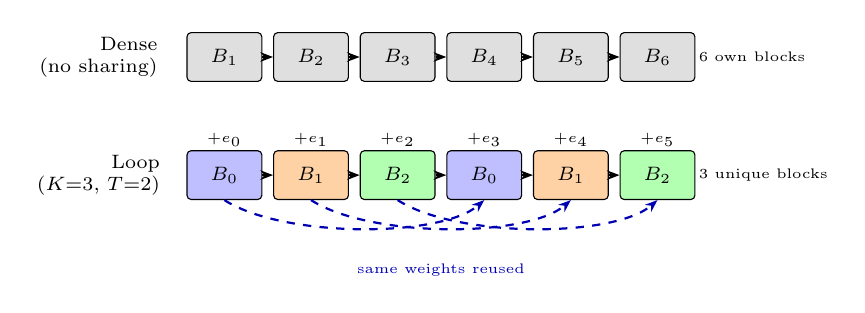
\begin{tikzpicture}[
  blk/.style={draw=black, rounded corners=1.5pt, minimum width=0.95cm, minimum height=0.62cm, font=\scriptsize, inner sep=1pt},
  lbl/.style={font=\scriptsize, align=right},
  arr/.style={-{Stealth[length=1.6mm]}, thick},
  shr/.style={-{Stealth[length=1.6mm]}, thick, dashed, blue!70!black}
]
% Dense: six blocks, six applications, each with its own weights
\node[lbl] at (-0.35,1.25) {Dense\\(no sharing)};
\foreach \i/\x in {1/1.25, 2/2.35, 3/3.45, 4/4.55, 5/5.65, 6/6.75} {
  \node[blk, fill=gray!25] (d\i) at (\x,1.25) {$B_{\i}$};
}
\foreach \i/\j in {1/2, 2/3, 3/4, 4/5, 5/6} {
  \draw[arr] (d\i) -- (d\j);
}
\node[font=\tiny, anchor=west] at (7.15,1.25) {6 own blocks};

% Loop: three unique blocks, each applied twice (T = 2), with a depth embedding before every application
\node[lbl] at (-0.35,-0.25) {Loop\\($K{=}3$, $T{=}2$)};
\node[font=\tiny] at (1.25,0.2) {$+e_0$};
\node[font=\tiny] at (2.35,0.2) {$+e_1$};
\node[font=\tiny] at (3.45,0.2) {$+e_2$};
\node[font=\tiny] at (4.55,0.2) {$+e_3$};
\node[font=\tiny] at (5.65,0.2) {$+e_4$};
\node[font=\tiny] at (6.75,0.2) {$+e_5$};
\node[blk, fill=blue!25]   (l1) at (1.25,-0.25) {$B_0$};
\node[blk, fill=orange!35] (l2) at (2.35,-0.25) {$B_1$};
\node[blk, fill=green!30]  (l3) at (3.45,-0.25) {$B_2$};
\node[blk, fill=blue!25]   (l4) at (4.55,-0.25) {$B_0$};
\node[blk, fill=orange!35] (l5) at (5.65,-0.25) {$B_1$};
\node[blk, fill=green!30]  (l6) at (6.75,-0.25) {$B_2$};
\foreach \i/\j in {1/2, 2/3, 3/4, 4/5, 5/6} {
  \draw[arr] (l\i) -- (l\j);
}
\draw[shr] (l1.south) .. controls (2.0,-1.05) and (4.0,-1.05) .. (l4.south);
\draw[shr] (l2.south) .. controls (3.1,-1.05) and (5.1,-1.05) .. (l5.south);
\draw[shr] (l3.south) .. controls (4.2,-1.05) and (6.2,-1.05) .. (l6.south);
\node[font=\tiny, blue!70!black] at (4.0,-1.45) {same weights reused};
\node[font=\tiny, anchor=west] at (7.15,-0.25) {3 unique blocks};
\end{tikzpicture}%
}

\caption{Dense versus cyclically shared depth (illustration with $K{=}3$ unique blocks and $T{=}2$ applications). A dense model applies six distinct blocks once each. A loop model applies its $K$ unique blocks cyclically over the depth slots, and a learned depth embedding $e_\ell$ is added before each application so that the shared block knows its slot. The experiments use $K{=}3$, $4$ and $6$, each with 12 layer applications per token.}
\label{fig:arch}
\end{figure}
\begin{table}[t]
\centering
\caption{Model family. Unique blocks $\times$ applications; ``Apps'' is layer applications per token. All models: $d{=}768$ unless noted, 12 heads, $d_{ff}{=}2048$, vocabulary 15{,}000, context 1{,}024.}
\label{tab:models}
\begin{tabular}{lcrr}
\toprule
Model & Blocks & Apps & Parameters \\
\midrule
Dense-12 & 12 & 12 & 96,473,856 \\
Dense-6 & 6 & 6 & 53,997,312 \\
Dense-4 & 4 & 4 & 39,838,464 \\
Dense-3 & 3 & 3 & 32,759,040 \\
Loop-6$\times$2 & 6 $\times$ 2 & 12 & 54,006,528 \\
Loop-4$\times$3 & 4 $\times$ 3 & 12 & 39,847,680 \\
Loop-3$\times$4 & 3 $\times$ 4 & 12 & 32,768,256 \\
Dense-12, $d{=}1024$ & 12 & 12 & 164,807,680 \\
Loop-6$\times$2, $d{=}1024$ & 6 $\times$ 2 & 12 & 90,096,640 \\
\bottomrule
\end{tabular}
\end{table}

\begin{table}[t]
\centering
\caption{Stored parameters, weight memory and forward compute per token. Weight memory is the parameter count stored in bfloat16 (2 bytes each). Forward GFLOPs count two operations per weight applied to a token, including the tied output projection; attention score products, which are the same for every 12-layer model of a given width, are excluded. Sharing reduces storage but not compute.}
\label{tab:memory}
\footnotesize
\setlength{\tabcolsep}{3pt}
\resizebox{\columnwidth}{!}{%
\begin{tabular}{lrrrr}
\toprule
Model & Unique params & Layers per token & Weights (MB) & Fwd GFLOPs \\
\midrule
Dense-12 & 96.5M & 12 & 192.9 & 0.193 \\
Dense-6 & 54.0M & 6 & 108.0 & 0.108 \\
Dense-4 & 39.8M & 4 & 79.7 & 0.080 \\
Dense-3 & 32.8M & 3 & 65.5 & 0.066 \\
Loop-6$\times$2 & 54.0M & 12 & 108.0 & 0.193 \\
Loop-4$\times$3 & 39.8M & 12 & 79.7 & 0.193 \\
Loop-3$\times$4 & 32.8M & 12 & 65.5 & 0.193 \\
Dense-12, $d{=}1024$ & 164.8M & 12 & 329.6 & 0.330 \\
Loop-6$\times$2, $d{=}1024$ & 90.1M & 12 & 180.2 & 0.330 \\
\bottomrule
\end{tabular}}
\end{table}

For shared models the same formula applies with the number of applications: each unique block is created once and initialised with $L=12$, not with its own count of six. Table~\ref{tab:init} compares the statistics at initialisation of Dense-6 and Loop-6$\times$2, measured on the first validation batch.
\begin{table}[t]
\centering
\caption{Statistics at initialisation (seed 0, first validation batch of four 1,024-token sequences). Dense-6 and Loop-6$\times$2 differ in the number of layer applications, so their output projections have different target scales (Section~\ref{sec:models}). Residual statistics are taken after the stated layer application; the gradient of a shared block is the sum over its applications.}
\label{tab:init}
\footnotesize
\setlength{\tabcolsep}{4pt}
\begin{tabular}{lrr}
\toprule
Quantity & Dense-6 & Loop-6$\times$2 \\
\midrule
Layer applications per token & 6 & 12 \\
Unique blocks & 6 & 6 \\
Output-projection std, target $0.02/\sqrt{2L}$ & 0.0058 & 0.0041 \\
Output-projection std, measured (block 0) & 0.0058 & 0.0041 \\
Residual std after application 1 & 0.048 & 0.061 \\
Residual std after last application & 0.162 & 0.285 \\
Residual variance after last application & 0.026 & 0.081 \\
Initial loss (nats) & 9.788 & 9.797 \\
Gradient norm, total & 10.086 & 21.936 \\
Gradient norm, mean per unique block & 3.775 & 8.486 \\
\bottomrule
\end{tabular}
\end{table}


\section{Data}
\label{sec:data}

\textbf{Corpus v1} has 1,151,073,280 training tokens in 275 shards and a validation split of 24.2M tokens in 6 shards. It is drawn from computer-science articles on Wikipedia, computer-science papers on arXiv, permissively licensed source code from The Stack~\cite{kocetkov2022stack}, and smaller documentation sources. Exact and MinHash~\cite{broder1997resemblance} near-duplicate removal ran before a document-level train/validation split. A byte-level byte-pair-encoding (BPE) tokenizer~\cite{sennrich2016bpe} with 15,000 tokens was trained on v1 and frozen.

\textbf{Corpus v2} adds 3,145,043,968 tokens from openly licensed public datasets, filtered for computer-science content by a keyword score with per-source caps: FineWeb-Edu~\cite{penedo2024fineweb} and Cosmopedia v2 (both via SmolLM-Corpus~\cite{smollmcorpus2024}), and Stack Exchange, arXiv and LibreTexts from the Common Pile~\cite{kandpal2025commonpile}. With the v1 shards copied in unchanged, v2 has 4,296,117,248 training tokens in 1,025 shards. It reuses the v1 tokenizer. A held-out split of 15.8M tokens (\texttt{val\_new}) comes from the new documents only.

\textbf{Document order} differs between the corpora. The v1 packer concatenates documents subject by subject, so each 4.19M-token v1 shard holds a single subject. The new v2 documents were shuffled globally before packing, so every new v2 shard mixes sources. Training visits the shards of a corpus in one fixed shuffled order, the same for every run on that corpus, and reads each shard sequentially.

\textbf{Benchmark decontamination.} During v2 construction, a document was dropped if it shared any 13-gram with a benchmark question (135 documents) or if 20\% or more of its 13-grams occurred in the v1 validation split (1,876 documents). A later full scan of all v1 and v2 training shards found no 13-gram from any of the 650 MMLU-CS questions. Exact 13-gram matching screens verbatim overlap only and does not detect paraphrased or translated items.

\subsection{Train--validation overlap audit}
\label{sec:overlap}

We matched every 13-token window of all 275 v1 training shards exactly against the windows of the 6 validation shards. 19.6\% of validation tokens lie inside at least one shared window, mostly licence headers and boilerplate. More seriously, 7.6\% lie inside verbatim runs of 100 or more tokens, which are copies of whole files; the longest is a 15,020-token source file. Document-level splitting after deduplication had not removed these cross-split copies.

On a 10\% sample of the new v2 shards (314.6M tokens), only 0.105\% of windows match validation and the longest shared run is 346 tokens (placeholder and licence text), against 3.13\% of windows and runs of up to 15,020 tokens in the same number of v1 training tokens. The new v2 documents therefore add almost no validation text.

We define the \emph{clean} tokens as the validation tokens outside verbatim runs of 100 or more tokens, and report every loss on both the full set and the clean tokens. Of the 3.02M target tokens in the evaluation subset (below), 2.81M are clean.

\section{Training and Evaluation}
\label{sec:setup}

\textbf{Training.} All models use AdamW~\cite{loshchilov2019adamw} with $\beta=(0.9,0.95)$, $\epsilon=10^{-8}$ and weight decay 0.1 on every parameter with at least two dimensions (this includes the depth embedding, which is initialised with standard deviation 0.02; normalisation gains are not decayed), gradient clipping at norm 1.0, and a cosine schedule with 2\% linear warmup (46 steps on v1, 171 on v2) that decays to 10\% of the peak learning rate (LR). The peak learning rate is $6\times10^{-4}$ for every $d=768$ model, with one extra run at $3\times10^{-4}$, and $5\times10^{-4}$ for the $d=1{,}024$ model. Each step uses 499,712 tokens (488 sequences of 1,024 tokens) via gradient accumulation. Training uses BF16 autocast with FP32 weights and optimizer state, in PyTorch~\cite{paszke2019pytorch}; later runs use \texttt{torch.compile}, which gave a 1.67$\times$ speedup with the same loss to four decimals. Every model trains for exactly one epoch: 2,302 steps on v1 and 8,595 steps on v2. Within each run, every token is seen at most once. Seed 1 sets the PyTorch seed to 1 (\texttt{-{}-seed 1}), whereas Seed 0 runs drew their PyTorch seed at random because no seed was passed; the data order is identical across runs on the same corpus (shuffle seed 0), so the second seed varies initialisation only. There is no dropout. Embedding and linear weights, other than the output projections and the depth embedding described above, are initialised from a normal distribution with standard deviation 0.02. The optimiser is AdamW in FP32 with BF16 autocast. Each step of 499,712 tokens is built from micro-batches of 8 sequences (4 for the width-1,024 models) by gradient accumulation; an out-of-memory handler halves the micro-batch while keeping the step size fixed. Gradients are clipped to a global norm of 1.0 before each update.

\textbf{Hardware.} All runs used one NVIDIA L4 (24 GB) graphics processing unit (GPU) on an Amazon Web Services (AWS) Elastic Compute Cloud (EC2) spot instance. Spot reclaims stop the instance; training saves a checkpoint on SIGTERM and a job queue resumes the run from its newest checkpoint on restart. About 250 GPU-hours were used in total (active training time from the run logs, with two first-regime runs estimated).

\textbf{Validation loss.} The reported metric is the mean token cross-entropy on every 8th batch of the v1 validation split (738 batches of $4\times1{,}024$ tokens, 3.02M target tokens), computed from the final checkpoint with a fresh data loader. Perplexity (PPL) is the exponential of this loss. The striding covers all validation subjects. Both corpora are evaluated on this same split.

\textbf{Multiple choice (MCQ).} We also report accuracy on 650 four-choice questions from six computer-science subjects of MMLU~\cite{hendrycks2021mmlu} (MMLU-CS). We use three likelihood rules, fixed before any result was seen. In the cloze rules the context is ``Question: \ldots\ Answer:'' and each continuation is the text of one choice; CF-sum picks the choice with the highest total log-likelihood and CF-norm, our primary rule, the highest log-likelihood per character. In the letter rule (MCF) the context also lists the four choices as ``A.~\ldots'' to ``D.~\ldots'', and the continuation is the answer letter. Every context starts with the document-separator token that precedes each document in training. For reference we also report the rule used by our training pipeline, which scores the mean loss of question plus choice. The answer key is not balanced (C is correct 28.8\% of the time, A 26.0\%), so we also check which letters each model predicts. Three baselines frame the results: uniform random choice (25.0\%), always answering C, the most frequent answer (28.8\%), and always answering A (26.0\%). Models should be compared with all three. A random-letter baseline has an expected accuracy of 25\%, with a sampling error of about 1.7 points on 650 questions.

\section{Results}

\subsection{One epoch on corpus v1}
\label{sec:v1}

\begin{table}[t]
\centering
\caption{Corpus v1 (1.15B tokens, one epoch, 2{,}302 steps). Validation loss in nats on the full strided subset and on the clean tokens (Section~\ref{sec:overlap}). Perplexity is on the full subset. MCQ is accuracy on the 650 MMLU-CS questions with the primary CF-norm rule (Table~\ref{tab:mcq}; chance 25\%, 95\% interval about $\pm$3.3 points). One seed per row.}
\label{tab:v1}
\setlength{\tabcolsep}{3pt}
\begin{tabular}{lrrrrrr}
\toprule
Model & Params & Apps & Val & Clean & PPL & MCQ \\
\midrule
Dense-12 & 96.5M & 12 & 2.853 & 2.914 & 17.3 & 26.9 \\
Dense-6 & 54.0M & 6 & 2.795 & 2.856 & 16.4 & 24.3 \\
Dense-4 & 39.8M & 4 & 2.998 & 3.058 & 20.0 & 27.2 \\
Dense-3 & 32.8M & 3 & 3.198 & 3.259 & 24.5 & 23.8 \\
Loop-6$\times$2 & 54.0M & 12 & 4.623 & 4.692 & 101.8 & 26.3 \\
Loop-6$\times$2 (LR 3e-4) & 54.0M & 12 & 4.592 & 4.660 & 98.7 & 23.7 \\
Loop-6$\times$2 (warmup 171) & 54.0M & 12 & 4.006 & 4.074 & 54.9 & 24.8 \\
Loop-4$\times$3 & 39.8M & 12 & 4.706 & 4.774 & 110.6 & 22.9 \\
Loop-3$\times$4 & 32.8M & 12 & 4.947 & 5.010 & 140.7 & 24.8 \\
\bottomrule
\end{tabular}
\end{table}

\begin{table}[t]
\centering
\caption{Matched-parameter comparison on corpus v1. Each loop model is paired with the dense model that has the same $K$ unique blocks and no sharing (unique parameters equal up to the 9{,}216-parameter depth embedding). Gap = loop $-$ dense validation loss (nats), on the full subset and on clean tokens. The last row is the warmup ablation: Loop-6$\times$2 with 171 instead of 46 warmup steps, everything else unchanged.}
\label{tab:gaps}
\begin{tabular}{crrrr}
\toprule
$K$ & Loop & Dense & Gap (full) & Gap (clean) \\
\midrule
6 & 4.623 & 2.795 & 1.83 & 1.84 \\
4 & 4.706 & 2.998 & 1.71 & 1.72 \\
3 & 4.947 & 3.198 & 1.75 & 1.75 \\
\midrule
6, warmup 171 & 4.006 & 2.795 & 1.21 & 1.22 \\
\bottomrule
\end{tabular}
\end{table}

\begin{figure}[t]
\centering
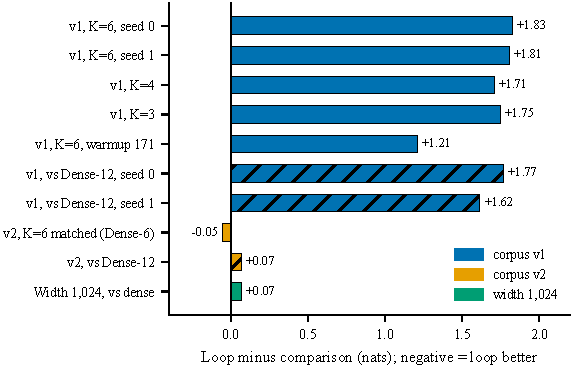
\includegraphics[width=\columnwidth]{figures/fig_gaps.pdf}
\caption{Loop-minus-comparison gaps in validation loss (full set). Solid bars compare with the parameter-matched dense control (first regime: $K{=}6$, $4$, $3$; second regime: $K{=}6$). Hatched bars compare with the 12-layer dense baseline at the same compute. The width-1,024 bar compares with the width-1,024 dense model, which has 1.8 times the loop's parameters.}
\label{fig:gaps}
\end{figure}


Table~\ref{tab:v1} reports all nine v1 runs, including the warmup ablation of Section~\ref{sec:ablation}, and Table~\ref{tab:gaps} pairs each loop model with its parameter-matched dense control. Every loop model is far worse than its control: 1.84 nats at $K=6$, 1.72 at $K=4$ and 1.75 at $K=3$ on clean tokens. The raw losses of the loop models are 4.69, 4.77 and 5.01 nats on clean tokens for $K=6$, 4 and 3, but these models also differ in size, so the matched gaps above are the comparison that matters. The compute-matched comparison is just as large: Loop-6$\times$2 (54.0M) is 1.78 nats worse than Dense-12 (96.5M), with the same 12 layer applications per token.

\subsection{What does not explain the gap}
\label{sec:causes}

\textbf{Parameter count.} The matched control holds the number of unique parameters fixed by design, so the gap is not a parameter-count effect by construction. The control does add one fact: Dense-6, with the same unique parameters as Loop-6$\times$2 and half its compute, is 1.84 nats better than the loop model and even slightly better than Dense-12 (2.856 against 2.914 nats on clean tokens). On this recipe, extra depth does not help dense models either.

\textbf{Learning rate.} Halving the peak learning rate of Loop-6$\times$2 changes its validation loss by $-0.03$ nats. The penalty is not an artifact of a learning rate tuned for dense models, at least within a factor of two.

\textbf{Overlap.} Re-scoring on clean tokens raises every loss by 0.06 to 0.07 nats and moves every gap by less than 0.01 nats.

\subsection{A second training regime (corpus v2)}
\label{sec:v2}

\begin{table}[t]
\centering
\caption{Second training regime (corpus v2: 4.30B tokens, one epoch, 8{,}595 steps, 171 warmup steps; the v1 tokens are a subset of v2). Validation loss in nats on the same v1 validation set. $\Delta$ = v2 clean $-$ v1 clean. The $d{=}1024$ rows have no v1 run. ``+ 2,048 context'' continues the $d{=}1024$ model for 400 steps at 2{,}048 tokens and is evaluated at 1{,}024 tokens. MCQ is CF-norm accuracy (\%, Table~\ref{tab:mcq}). One seed per row.}
\label{tab:v2}
\setlength{\tabcolsep}{2.8pt}
\begin{tabular}{lrrrrrr}
\toprule
Model & Params & v1 clean & v2 val & v2 clean & $\Delta$ & MCQ \\
\midrule
Dense-12 & 96.5M & 2.914 & 2.015 & 2.072 & $-0.84$ & 27.4 \\
Loop-6$\times$2 & 54.0M & 4.692 & 2.084 & 2.140 & $-2.55$ & 26.8 \\
Dense-6 & 54.0M & 2.856 & 2.135 & 2.192 & $-0.66$ & 25.5 \\
Dense-12, $d{=}1024$ & 164.8M & -- & 1.927 & 1.986 & -- & 26.0 \\
\quad + 2,048 context & 164.8M & -- & 1.924 & 1.983 & -- & 26.2 \\
Loop-6$\times$2, $d{=}1024$ & 90.1M & -- & 1.999 & 2.057 & -- & 26.5 \\
\bottomrule
\end{tabular}
\end{table}

\begin{table}[t]
\centering
\caption{Clean validation loss (nats) of the two v2 runs at periodic checkpoints, scored with the official protocol. Step 8{,}595 is the final checkpoint. The last row is the end of the v1 runs, for comparison at a similar step count.}
\label{tab:curve}
\begin{tabular}{rrrr}
\toprule
Step & Dense-12 & Loop-6$\times$2 & Gap \\
\midrule
400 & 4.451 & 5.212 & $+0.762$ \\
1,200 & 2.694 & 2.807 & $+0.113$ \\
2,400 & 2.479 & 2.560 & $+0.081$ \\
4,000 & 2.278 & 2.345 & $+0.067$ \\
6,000 & 2.141 & 2.204 & $+0.063$ \\
8,000 & 2.078 & 2.145 & $+0.067$ \\
8,595 & 2.072 & 2.140 & $+0.068$ \\
\midrule
v1 end (2,302) & 2.914 & 4.692 & $+1.778$ \\
\bottomrule
\end{tabular}
\end{table}

\begin{figure}[t]
\centering
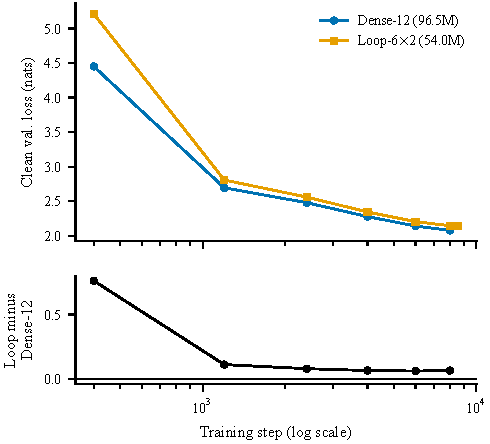
\includegraphics[width=\columnwidth]{figures/fig_curve_v2.pdf}
\caption{Clean validation loss of the two second-regime runs at periodic checkpoints (top) and the loop-minus-dense gap over training (bottom). The gap is 0.76 nats at step 400, about 0.07 nats from step 4,000 on, and 1.78 nats at the end of the first regime (step 2,302).}
\label{fig:curve}
\end{figure}

\begin{table}[t]
\centering
\caption{Corpus v2: mean token loss (nats) per validation shard, on the strided batches of the official evaluation. The gap is nearly constant across shards.}
\label{tab:shards}
\begin{tabular}{crrr}
\toprule
Shard & Dense-12 & Loop-6$\times$2 & Gap \\
\midrule
0 & 2.146 & 2.214 & $+0.068$ \\
1 & 1.461 & 1.522 & $+0.061$ \\
2 & 1.623 & 1.685 & $+0.062$ \\
3 & 1.532 & 1.595 & $+0.063$ \\
4 & 2.615 & 2.697 & $+0.082$ \\
5 & 2.923 & 3.006 & $+0.083$ \\
\bottomrule
\end{tabular}
\end{table}


Table~\ref{tab:v2} shows the completed v2 runs; the width-1,024 rows are discussed below. On clean tokens Dense-12 improves by 0.84 nats, Dense-6 by 0.66 and Loop-6$\times$2 by 2.55. The compute-matched gap (Loop-6$\times$2 against Dense-12) falls from 1.78 nats on v1 to 0.07 nats on v2. At matched parameters the sign flips: Loop-6$\times$2 is 0.052 nats better than Dense-6 on v2 (2.140 against 2.192), where it was 1.84 nats worse on v1. With the same unique parameters, the shared model now turns its twice-larger compute into a lower loss.

Table~\ref{tab:curve} shows that this is not a matter of training for more steps. We scored the periodic checkpoints of both v2 runs with the official protocol. The gap is 0.76 nats at step 400, 0.11 at step 1,200 and 0.08 at step 2,400, which is about the length of the v1 runs, and then stays between 0.06 and 0.07 nats. Step 2,400 is about 1.2 billion tokens (2,400 steps of 499,712 tokens), so this is an equal-token comparison with the 1.15 billion tokens of the first regime. It is not an equal-learning-rate comparison: at that step the learning rate is about 85\% of its peak, while the first regime has decayed to 10\%. For the compute-matched pair (Loop-6$\times$2 and Dense-12, which both apply 12 layers per token), equal tokens also mean equal FLOPs; for the parameter-matched pair they do not, because the loop model applies its blocks twice as often. At a similar step count, the v1 runs ended 1.78 nats apart. At step 2,400 of the v2 schedule the learning rate is still close to its peak, while the v1 runs had decayed to 10\% of it; decay usually lowers the loss, so this comparison, if anything, favours v1. Table~\ref{tab:shards} shows that the final v2 gap is also uniform across the validation text: between 0.061 and 0.083 nats in every shard, and between 0.057 and 0.084 nats in every tenth of the validation stream.

The training logs agree. On v1, the loop models fall behind their dense controls within the first 100 steps and never recover, although all v1 runs saw the same data in the same order: the mean training loss over steps 400 to 800 is 4.74 for Dense-6, against 5.72 for Loop-6$\times$2 (learning rate $3\times10^{-4}$) and 6.19 for Loop-3$\times$4. On v2 the loop model also starts behind the dense baseline but has nearly caught up by step 1,200.

\textbf{What differs between the regimes.} The two regimes differ in four ways at once: warmup length (46 against 171 steps, because warmup is 2\% of the schedule), schedule length (the learning rate decays over 2,302 against 8,595 steps), data mix (v2 adds 3.1B tokens of web, question-answer, synthetic and paper text), and document order (single-subject v1 shards against source-mixed v2 shards). The v2 runs alone cannot separate these factors; the ablation below isolates the first.

\subsection{Warmup ablation}
\label{sec:ablation}

To test the first factor we reran Loop-6$\times$2 on v1 with 171 warmup steps instead of 46, the same warmup as the v2 runs, and changed nothing else: same data, same order, same peak learning rate and the same 2,302 steps (last row of Table~\ref{tab:gaps}, and Table~\ref{tab:v1}). The longer warmup lowers its clean validation loss from 4.692 to 4.074 nats. This recovers 0.62 of the 1.84-nat gap to Dense-6, about a third; 1.22 nats remain on clean tokens. Warmup is therefore part of the cause, but most of the v1 penalty comes from the other differences between the regimes: schedule length, data mix or document order. On MMLU-CS the ablated model is at chance (24.8\%), like every other model.

\subsection{Width and seeds}

\textbf{Width.} At $d=1{,}024$ (16 heads, $d_{ff}=2{,}688$, 164.8M parameters, peak learning rate $5\times10^{-4}$), the 12-layer dense model trained on v2 reaches 1.927 nats (1.986 on clean tokens), 0.086 nats below the 96.5M dense model on clean tokens (Table~\ref{tab:v2}). Continuing it for 400 steps at a 2,048-token context (peak learning rate $10^{-4}$) changes the loss at 1,024 tokens by $-0.003$ nats; our evaluation uses 1,024-token sequences, so it does not measure what the longer context adds. Both width-1,024 models stay at chance on MMLU-CS. The width-1,024 loop model (90.1M parameters, peak learning rate $5\times10^{-4}$) reaches 1.999 nats (2.057 on clean tokens): 0.072 nats above the width-1,024 dense model (full set), which has 1.8 times its parameters, and 0.016 nats below the 96.5M dense baseline, which uses about 1.8 times less compute per token. Its CF-norm accuracy is 26.5\%.
\begin{table}[t]
\centering
\caption{Second seed on corpus v1. Validation loss (nats, full set) for seed 0 and seed 1, the change between seeds. The gap rows are loop minus the comparison model, for each seed.}
\label{tab:seeds}
\setlength{\tabcolsep}{4pt}
\begin{tabular}{lrrr}
\toprule
Model / gap & Seed 0 & Seed 1 & Change \\
\midrule
Dense-12 & 2.853 & 2.887 & $+0.034$ \\
Dense-6 & 2.795 & 2.697 & $-0.098$ \\
Loop-6$\times$2 & 4.623 & 4.502 & $-0.120$ \\
\midrule
Gap, matched (vs Dense-6) & 1.827 & 1.805 & $-0.022$ \\
Gap, compute (vs Dense-12) & 1.769 & 1.616 & $-0.154$ \\
\bottomrule
\end{tabular}
\end{table}

\textbf{Second seed.} Table~\ref{tab:seeds} repeats the first-regime runs with a second seed. Single-model losses move by 0.03 nats (Dense-12), 0.10 (Dense-6) and 0.12 (Loop-6$\times$2) between seeds. The matched gap (loop minus Dense-6) is 1.83 nats on seed 0 and 1.81 on seed 1, so it is stable. The compute-matched gap (loop minus Dense-12) is 1.77 and 1.62, a spread of 0.15 nats, so the first-regime compute-matched penalty should be read as 1.6 to 1.8 nats. For the second regime, the baseline's second seed differs from its first by only 0.005 nats. No second seed was run for the matched v2 pair, so the 0.05-nat reversal remains a single-seed result.

Table~\ref{tab:paired} gives the seed means and the paired differences. Its last column is the paired difference on a CPU subsample of the official validation batches, with a 95\% interval from resampling batches of four sequences; the weights of the first-seed runs are no longer stored, so the seed-0 gaps have no interval.
\begin{table}[t]
\centering
\caption{Two seeds, first regime (full validation set, official values) and second regime (Dense-12, two seeds). Gaps are loop minus the comparison model, per seed. The last column gives the paired difference on the CPU subsample with a 95\% interval from resampling batches of four sequences (every 8th official batch, 93 of the 738 batches; Section~\ref{sec:setup}). Intervals reflect sampling of batches, not seed variation. Batch-level bootstrap intervals ignore correlation between batches from the same document or subject, so they likely underestimate uncertainty.}
\label{tab:paired}
\footnotesize
\setlength{\tabcolsep}{3pt}
\resizebox{\columnwidth}{!}{%
\begin{tabular}{lrrrl}
\toprule
Model / gap & Seed 0 & Seed 1 & Mean & Subsample diff. [95\% CI] \\
\midrule
Dense-12, v1 & 2.853 & 2.887 & 2.870 & -- \\
Dense-6, v1 & 2.795 & 2.697 & 2.746 & -- \\
Loop-6$\times$2, v1 & 4.623 & 4.502 & 4.562 & -- \\
\midrule
Matched gap (loop $-$ Dense-6) & 1.827 & 1.805 & 1.816 & +1.753 [+1.656, +1.851] \\
Compute gap (loop $-$ Dense-12) & 1.769 & 1.616 & 1.692 & +1.567 [+1.472, +1.666] \\
\midrule
Dense-12, v2 & 2.015 & 2.009 & 2.012 & -- \\
Matched gap, v2 (loop $-$ Dense-6) & $-$0.052 & -- & -- & $-$0.052 [$-$0.055, $-$0.048] \\
Compute gap, v2 (loop $-$ Dense-12) & 0.069 & 0.074 & 0.072 & +0.068 [+0.064, +0.073] \\
\bottomrule
\end{tabular}}
\end{table}


\begin{figure}[t]
\centering
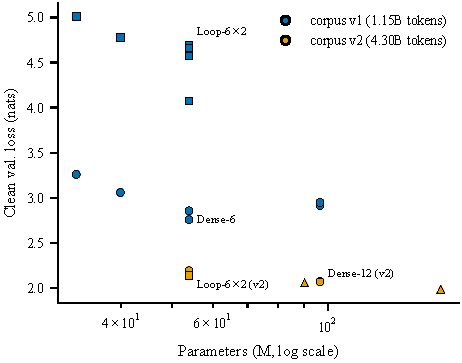
\includegraphics[width=\columnwidth]{figures/fig_scatter.pdf}
\caption{Clean validation loss against parameter count for all runs. Circles: dense; squares: loop; triangles: width 1,024. Blue: corpus v1; orange: corpus v2. Losses from the two corpora are not directly comparable, because the validation split and training data differ.}
\label{fig:scatter}
\end{figure}
Figure~\ref{fig:pareto} plots clean validation loss against the memory needed for the weights in bfloat16. Error bars span the two seeds where both exist, and dashed lines mark the Pareto front within each corpus.
\begin{figure}[t]
\centering
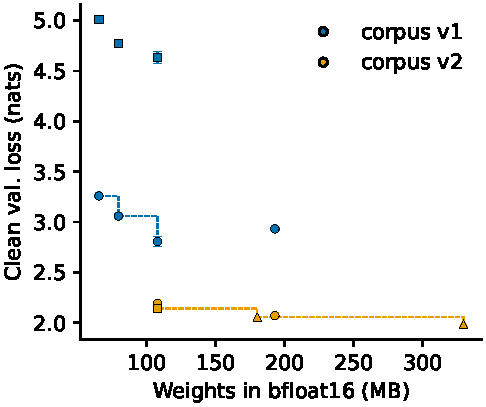
\includegraphics[width=\columnwidth]{figures/fig_pareto.pdf}
\caption{Clean validation loss against weight memory in bfloat16, for every configuration. Circles: dense; squares: loop; triangles: width 1,024. Error bars span the two seeds where both exist. Dashed lines: Pareto front within each corpus. The two corpora are not directly comparable.}
\label{fig:pareto}
\end{figure}

\subsection{Multiple choice}

\begin{table}[t]
\centering
\caption{Accuracy (\%) on the 650 MMLU-CS questions under four scoring rules. ``Old'' is the mean loss of question plus choice; CF-norm (primary, fixed before results) and CF-sum are the cloze log-likelihood of the choice given the question, per character and in total; MCF is the log-likelihood of the answer letter. ``A\%'' is how often MCF picks A. Chance is 25\%; always answering C scores 28.8\% and always A 26.0\%. The 95\% interval is about $\pm$3.3 points.}
\label{tab:mcq}
\setlength{\tabcolsep}{3.5pt}
\begin{tabular}{lrrrrr}
\toprule
Model & Old & CF-norm & CF-sum & MCF & A\% \\
\midrule
Dense-12 & 26.9 & 26.9 & 24.3 & 26.3 & 91 \\
Dense-6 & 25.5 & 24.3 & 23.2 & 26.8 & 86 \\
Dense-4 & 26.3 & 27.2 & 22.6 & 25.4 & 82 \\
Dense-3 & 27.5 & 23.8 & 23.8 & 26.3 & 98 \\
Loop-6$\times$2 & 28.6 & 26.3 & 24.3 & 26.2 & 100 \\
Loop-6$\times$2 (LR 3e-4) & 24.2 & 23.7 & 24.6 & 26.0 & 100 \\
Loop-6$\times$2 (warmup 171) & 25.4 & 24.8 & 25.8 & 25.7 & 98 \\
Loop-4$\times$3 & 26.6 & 22.9 & 25.5 & 25.8 & 100 \\
Loop-3$\times$4 & 27.8 & 24.8 & 24.8 & 26.0 & 100 \\
Dense-12, seed 1 & 27.7 & 26.8 & 23.8 & 24.3 & 80 \\
Dense-6, seed 1 & 27.7 & 24.0 & 23.7 & 26.3 & 96 \\
Loop-6$\times$2, seed 1 & 26.5 & 25.7 & 23.7 & 26.3 & 100 \\
Dense-12 (v2) & 25.7 & 27.4 & 24.6 & 25.2 & 91 \\
Dense-12, seed 1 (v2) & 28.3 & 27.8 & 25.8 & 25.4 & 98 \\
Loop-6$\times$2 (v2) & 27.5 & 26.8 & 24.2 & 25.4 & 94 \\
Dense-6 (v2) & 28.2 & 25.5 & 25.8 & 26.2 & 89 \\
Dense-12, $d{=}1024$ (v2) & 27.7 & 26.0 & 22.3 & 25.1 & 90 \\
\quad + 2,048 context & 28.5 & 26.2 & 23.1 & 24.9 & 92 \\
Loop-6$\times$2, $d{=}1024$ (v2) & 26.6 & 26.5 & 24.9 & 25.5 & 94 \\
\bottomrule
\end{tabular}
\end{table}

\begin{figure}[t]
\centering
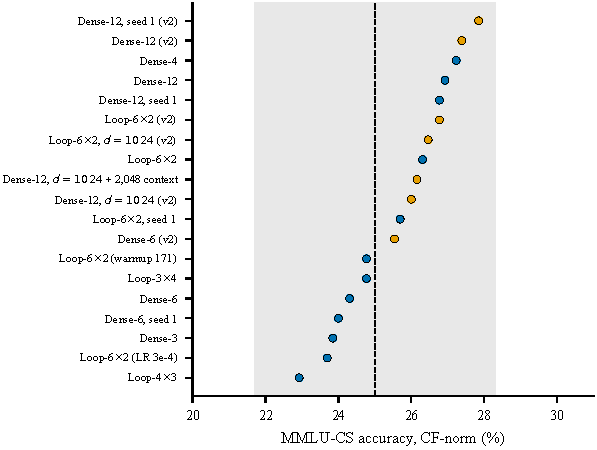
\includegraphics[width=\columnwidth]{figures/fig_mcq.pdf}
\caption{Conditional-likelihood (CF-norm) accuracy on the 650 MMLU-CS questions for all 19 runs. Dashed line: chance (25\%). Shaded band: 95\% interval ($\pm$3.3 points). Every run lies inside the band.}
\label{fig:mcq}
\end{figure}


Table~\ref{tab:mcq} reports MMLU-CS under all four rules (three likelihood rules and the reference rule of the training pipeline). With the primary rule (CF-norm) the nineteen completed runs score between 22.9\% and 27.8\%; the best is 1.7 standard errors above chance, which is not significant. The letter rule shows a strong position bias: every model answers ``A'' on 80\% to 100\% of the questions, so its accuracy is essentially that of always answering A (26.0\%). Paired on the same questions, the v1 and v2 versions of each model do not differ (McNemar $\chi^2=0.03$ for both Dense-12 and Loop-6$\times$2), although their validation losses differ by 0.84 and 2.55 nats. The benchmark therefore does not separate the models at this scale under any of the rules, and validation loss remains the informative metric. We keep MMLU-CS in the evaluation because it is the standard test for the domain and it will become informative at larger scale.

\section{Discussion}

The v1 result, a 1.7 to 1.8 nat penalty for sharing that neither parameter count nor learning rate explains, does not survive a change of training regime. In the second regime the shared model is within 0.08 nats of the compute-matched dense model at a similar step count, and it beats the dense model with the same unique parameters. The v1 penalty is therefore neither the steady-state cost of sharing nor simply a matter of training longer. Something in the first regime hurts the shared models far more than the dense ones, even though both saw identical data in identical order.

We had two hypotheses. First, a shared block's gradient is the sum over all the depth slots that use it, and early in training these contributions may disagree, a form of gradient conflict that has been studied in multi-task learning~\cite{chai2023gradient,chen2025expert,xiong2026qmate}; a 46-step warmup to the peak learning rate may move the shared weights into a poor region from which they do not fully recover. The ablation supports this only in part: a 171-step warmup recovers about a third of the penalty. Second, single-subject shards turn training into a sequence of long, homogeneous blocks, which may pull weights that serve every depth back and forth more than per-layer weights. Halving the peak learning rate did not help on v1, which argues against the peak step size alone. The remaining two thirds of the penalty may come from the schedule length, the data mix or the document order. A source-shuffled v1 ablation would test the document-order part of this; we have not run it.

The practical lesson holds either way. The two recipes give compute-matched gaps that differ by more than twenty-fold (1.78 against 0.08 nats at a similar step count), so a single-recipe comparison can badly misestimate the cost of sharing. Studies of sharing schemes should vary the recipe, or at least report warmup length and data order, before concluding that sharing hurts.

\section{Limitations}

Most configurations have one seed; the three first-regime runs (Dense-12, Dense-6 and Loop-6$\times$2) have a second seed, and so does the second-regime Dense-12 baseline. The scale is small (at most 164.8M parameters on completed runs) and the domain is one: computer science. The learning rate was tuned for the dense baseline and checked at one alternative for the loop model, not swept. The two training regimes differ in warmup length, schedule length, data mix and document order at once; the warmup ablation isolates only the first, and the other three are not separated. The dense controls are matched on parameters, not compute, and only the 12-layer dense model is compute-matched. We tested one conditioning scheme for shared blocks (an additive depth embedding). Under the second recipe we ran only $K=6$, so the comparison over $K$ exists only under the first recipe. Multiple-choice accuracy is at chance for every model under every rule we tried, so at this scale the benchmark does not measure differences between models. Finally, the in-training validation values logged during training are not comparable across evaluations because the loader position carried over between them; all reported numbers come from the separate final evaluation. The source-shuffled v1 ablation, a learning-rate sweep for the loop model and a second seed for the matched v2 pair are left for future work. The depth-conditioning alternatives (no embedding, sinusoidal, gated and zero-initialised embeddings), gradient interference across depth positions (RQ2), latency and throughput, and independent held-out validation sets were not measured or collected. The intervals in Table~\ref{tab:paired} resample batches of four sequences on a subsample of the official validation batches; they do not capture seed-to-seed variation, which is reported separately. The output-projection scale difference between Dense-6 and Loop-6$\times$2 (Section~\ref{sec:models}) is uncontrolled. The second-seed comparison varies model initialisation only, with data order held fixed.

\section{Conclusion}

For small decoder-only models trained from scratch on a computer-science corpus, cyclic depth-wise weight sharing cost 1.7 to 1.8 nats of validation loss after one epoch of 1.15B tokens in our first training regime, at matched parameters and at matched compute. In a second regime, with a longer warmup, a longer schedule and a larger, source-mixed corpus, the compute-matched cost is 0.08 nats at a similar step count and 0.07 nats at the end, and at matched parameters the shared model is 0.05 nats better than the dense one. A longer warmup alone recovers about a third of the first-regime penalty. The cost of sharing therefore depends strongly on the training recipe, and a single short-recipe comparison should not be read as the cost of sharing itself. A second seed confirms the first-regime matched gap (1.81 against 1.83 nats), while compute-matched gaps vary by 0.15 nats between seeds. The second-regime reversal (0.05 nats) is a single-seed result and is reported as provisional. The second-regime result is thus an encouraging indication that cyclic depth-wise weight sharing may be competitive with (and potentially surpass) a dense baseline under some favorable training conditions. However, as this observation is based on a single seed, further multi-seed experiments and statistical verification are required to make strong claims about its superiority.

\section{Reproducibility}

The AstraCSE code, configurations, data pipelines, overlap audit and table-generation scripts are available at \url{https://github.com/bhargav-abhay/AstraCSE-Looped-Transformers}. The repository includes a SHA-256 manifest of the configuration and result files (paper/data/MANIFEST.sha256); hashes of the model weight files are available on request. Tables are produced by \texttt{paper/make\_tables.py} from the official evaluation files.

\section*{Acknowledgment}

Experiments ran on AWS EC2 spot instances.

\bibliographystyle{IEEEtran}
\bibliography{references}

\end{document}
